\begin{proof}
    To disprove the statement I just have to find a counterexample.\par
    Let \(f\) be a function defined on \([-1,1]\) with values in the extended reals. Specifically:
    \begin{align*}
        f:[-1,1] &\rightarrow \R \cup \{\pm\infty\} \\
        x &\mapsto -x^2 + 1
    \end{align*}
    Clearly, \(f\) is not a convex function (a quadratic function is convex if its quadratic coefficient is greater than or equal to zero). Therefore, the epigraph of the function \(P(f)\) is not a convex set (by definition of convex function).
    \begin{figure}
        \centering
        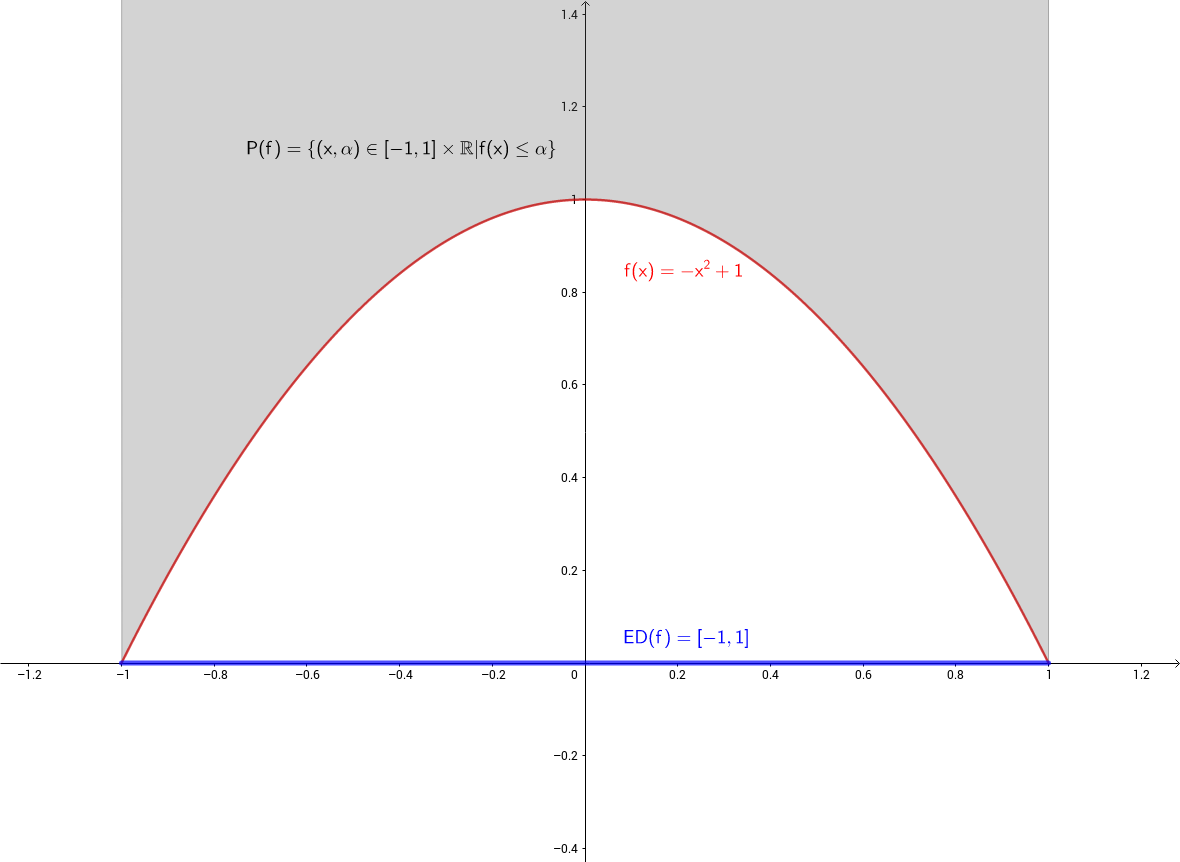
\includegraphics[width=0.9\textwidth]{../Images/epigraph_effectivedomain.png}
        \caption{Graphical representation of the function \(f(x) = -x^2 + 1\), its epigraph \(P(f)\) and its effective domain \(ED(f)\)}
        \label{epigraph_effectivedomain}
    \end{figure}
    A graphical representation of the epigraph (see figure \ref{epigraph_effectivedomain}) is useful to see that the set is not convex.\par
    Let's now take into account the effective domain of \(f\). Recall that \(ED(f)\) is the projection of \(P(f)\):
    \[ED(f) = [-1,1]\]
    The effective domain of \(f\) is clearly a convex set (the line segment between any two points of \(ED(f)\) lies in \(ED(f)\), since \(ED(f)\) is a segment line). We can conclude that, in this specific case, the statement does not hold (\(ED(f)\) is a convex set, \(P(f)\) is not). Thus, the statement does not always hold.
\end{proof}